\documentclass[12pt]{article}

\usepackage{sbc-template}
\usepackage{graphicx,url}
\usepackage[utf8]{inputenc}
\usepackage[brazil]{babel}     
\usepackage{float}

\sloppy

\title{Trabalho Prático\\ Ferramenta de Processamento de Dados com Grafos}

\author{Áulus Batista\inst{1}, Davi Soares\inst{1}, Henrique Neves\inst{1}, Pedro Matos\inst{1}, \\Maria Clara Gomes\inst{1}, Vinícius Simões\inst{1}}

\address{\small Instituto de Ciências Exatas e Informática (ICEI) -- Pontifícia Universidade Católica de Minas Gerais \\(PUC Minas)
Campus Coração Eucarístico (Coreu) -- Belo Horizonte -- MG -- Brazil\\
{\small E-mails: aulus.batista, davi.soares, henrique.neves, pedro.matos, maria.clara, \\vinicius.simoes@sga.pucminas.br}
}

\begin{document} 

\maketitle

\begin{abstract}
This paper presents the development and evaluation of a Python tool for
urban route planning using a directed, weighted graph. The tool
implements Dijkstra's and Bellman-Ford algorithms and allows the user
to select distance, estimated travel time, or estimated fuel cost as
the optimization criterion. The evaluation used a local OpenStreetMap
snapshot of the Coração Eucarístico neighborhood in Belo Horizonte,
containing 34 vertices and 68 directed edges. Both algorithms were
evaluated on 1,122 ordered vertex pairs, with 20 timed repetitions for
each pair and criterion. They returned equal route costs in the
evaluated queries. Dijkstra had lower median execution times for all
three criteria in this snapshot. These measurements describe a small
graph and should not be generalized to larger road networks.
\end{abstract}

\begin{resumo}
Este artigo apresenta o desenvolvimento e a avaliação de uma ferramenta
em Python para planejamento de rotas urbanas por meio de um grafo
direcionado e ponderado. A ferramenta implementa os algoritmos de
Dijkstra e Bellman-Ford e permite selecionar distância, tempo estimado
ou custo financeiro estimado como critério de otimização. A avaliação
utilizou um snapshot local do OpenStreetMap referente ao bairro Coração
Eucarístico, em Belo Horizonte, com 34 vértices e 68 arestas
direcionadas. Os algoritmos foram avaliados em 1.122 pares ordenados de
vértices, com 20 medições para cada par e critério. Ambos retornaram
custos iguais nas consultas avaliadas. Nesse snapshot, Dijkstra
apresentou menores medianas de tempo nos três critérios. Como o grafo
avaliado é pequeno, esses resultados não devem ser generalizados para
redes viárias maiores.
\end{resumo}

\section{Introdução}
\label{sec:introducao}
A busca por rotas em ambientes urbanos pode ser tratada como um
problema de caminho mínimo em grafos. Nessa representação, os
cruzamentos e outros pontos da rede viária são modelados como vértices,
enquanto os trechos de via são representados por arestas. Associar
pesos às arestas permite calcular percursos segundo diferentes
critérios, como distância, tempo estimado de deslocamento ou custo
financeiro.

Este trabalho apresenta uma ferramenta computacional para calcular
rotas urbanas usando os algoritmos de Dijkstra e Bellman-Ford. A
aplicação permite que o usuário informe a origem e o destino, selecione
um critério de otimização e escolha qual algoritmo será executado. Os
resultados são exibidos em uma interface com mapa, caminho encontrado e
métricas da rota.

A ferramenta foi desenvolvida em Python e utiliza um grafo direcionado
e ponderado construído a partir de dados locais do OpenStreetMap. O
snapshot usado na avaliação corresponde a um recorte do bairro Coração
Eucarístico, em Belo Horizonte, com 34 vértices e 68 arestas
direcionadas. Embora a aplicação tenha como contexto o roteamento em
Belo Horizonte, os experimentos deste artigo se limitam a essa malha
local.

A avaliação compara os dois algoritmos em 1.122 pares ordenados de
vértices, considerando os critérios de distância, tempo estimado e
custo financeiro. Para cada combinação de par, critério e algoritmo,
foram realizadas 20 medições cronometradas, após uma execução de
aquecimento. Os resultados mostraram custos de rota iguais entre os
algoritmos nas consultas avaliadas e menores medianas de tempo para
Dijkstra nesse snapshot. Como a rede analisada é pequena, os resultados
caracterizam apenas o conjunto de dados e o ambiente utilizados.

O restante do artigo está organizado da seguinte forma: a
Seção~\ref{sec:objetivo} apresenta os objetivos; a
Seção~\ref{sec:fundamentacao} discute os conceitos e trabalhos
relacionados; a Seção~\ref{sec:metodologia} descreve as etapas de
desenvolvimento; a Seção~\ref{sec:dados} caracteriza os dados e o
problema; a Seção~\ref{sec:modelagem} apresenta a modelagem; e a
Seção~\ref{sec:algoritmo} detalha os algoritmos e a implementação. A
Seção~\ref{sec:interface} apresenta a aplicação, a
Seção~\ref{sec:avaliacao} descreve o protocolo e os resultados, e a
Seção~\ref{sec:discussao} discute os achados e as limitações. Por fim,
a Seção~\ref{sec:conclusao} apresenta as conclusões e os trabalhos
futuros.
\section{Objetivo}
\label{sec:objetivo}
Desenvolver uma ferramenta computacional para resolver o problema de otimização de rotas urbanas com base em mapas, aplicado por meio
da modelagem, implementação e análise de grafos.
\subsection{Objetivos específicos}
\begin{itemize}
    \item Importar e processar mapas estruturados contendo pontos de interesse;
    \item Modelar a rede viária e os custos de deslocamento por meio de grafos;
    \item Implementar algoritmos de caminho mínimo para o cálculo e a exibição de rotas otimizadas;
    \item Comparar Dijkstra e Bellman-Ford quanto aos custos retornados, ao tempo de execução e à quantidade de vértices processados no snapshot avaliado;
\end{itemize}

\section{Fundamentação Teórica}
\label{sec:fundamentacao}

Um grafo direcionado e ponderado pode ser definido como
$G=(V,E,w)$, em que $V$ representa o conjunto de vértices, $E$ o
conjunto de arestas direcionadas e $w$ atribui um peso a cada aresta.
Em uma rede viária, os vértices representam posições da malha, como
cruzamentos, e as arestas representam trechos percorridos entre essas
posições. A direção das arestas permite representar vias de mão única,
enquanto duas arestas em sentidos opostos representam um trecho
percorrível nos dois sentidos. Os pesos podem expressar distância,
tempo ou outro custo associado ao deslocamento \cite{cormen2009}.

Para um caminho $P$ formado por uma sequência de arestas, seu custo é
a soma dos pesos das arestas percorridas:
\[
    w(P)=\sum_{e \in P} w(e).
\]
O problema de caminho mínimo consiste em encontrar, entre uma origem e
um destino, um caminho cujo custo total seja mínimo segundo o peso
selecionado.

O algoritmo de Dijkstra resolve esse problema quando os pesos das
arestas são não negativos. A cada etapa, seleciona o vértice alcançável
com a menor estimativa de custo e relaxa suas arestas de saída. A
relaxação atualiza a estimativa do vértice de destino quando o caminho
encontrado por aquela aresta é menor que o custo conhecido. Com uma
fila de prioridade, a implementação evita procurar linearmente pelo
próximo vértice de menor custo \cite{cormen2009}.

O algoritmo de Bellman-Ford também calcula caminhos mínimos por meio
da relaxação das arestas. Em vez de selecionar o próximo vértice por
uma fila de prioridade, realiza passadas sucessivas pelas arestas
alcançáveis. São necessárias, no máximo, $|V|-1$ passadas para
determinar os menores custos quando não há ciclos de peso negativo
alcançáveis. Uma passada adicional pode detectar esses ciclos
\cite{sedgewick2011}. Embora Bellman-Ford possa trabalhar com arestas
de peso negativo, os pesos aceitos pelo modelo deste sistema são
não negativos.

\subsection{Trabalhos Relacionados}

Trabalhos sobre roteamento em redes viárias de grande escala estudam
técnicas de aceleração, como hierarquização e pré-processamento de
rotas, para reduzir o tempo de consulta em redes extensas
\cite{bast2016}. O presente projeto tem escopo diferente: implementa
Dijkstra e Bellman-Ford sem essas etapas de aceleração, permite que o
usuário selecione o algoritmo e compara os resultados em um snapshot
local pequeno. Assim, a avaliação caracteriza a implementação e os
dados utilizados, mas não reproduz as condições de roteamento de uma
malha urbana completa.
\section{Metodologia}
\label{sec:metodologia}

Este trabalho tem caráter aplicado e compreende o desenvolvimento de
uma ferramenta de roteamento urbano e a avaliação experimental de dois
algoritmos de caminho mínimo. O processo foi organizado em etapas:
definição dos requisitos, preparação dos dados, modelagem da rede,
implementação da aplicação e avaliação dos resultados. As etapas são
apresentadas nesta seção; os detalhes do conjunto de dados, dos
diagramas, dos algoritmos e do protocolo experimental são descritos nas
seções seguintes.

\subsection{Definição dos requisitos}

Inicialmente, foram definidos os dados de entrada e as funcionalidades
esperadas. A aplicação deve permitir a seleção de origem e destino, do
critério de otimização e do algoritmo de busca. Os critérios
considerados são distância, tempo estimado e custo financeiro; os
algoritmos disponíveis são Dijkstra e Bellman-Ford. O sistema também
deve apresentar o caminho encontrado e as métricas calculadas para a
rota.

\subsection{Preparação e modelagem dos dados}

A malha viária foi representada como um grafo direcionado e ponderado.
Os dados do snapshot local do OpenStreetMap foram armazenados em JSON e
convertidos para a estrutura de grafo utilizada pelo programa. Os
trechos de mão dupla são representados por arestas nos dois sentidos,
enquanto as vias de mão única mantêm apenas a direção registrada.

Também foi utilizado um catálogo local de pontos de interesse. A
interface oferece consultas ao Nominatim para buscar ou geocodificar
locais, mas essas consultas não fazem parte do benchmark, que utiliza
diretamente os vértices do grafo local. A delimitação e as
características dos dados são apresentadas na Seção~\ref{sec:dados}.

\subsection{Implementação e integração}

Após a modelagem, foram implementadas as classes de representação do
grafo e os algoritmos de busca em Python. A interface foi construída
com Streamlit e apresenta o mapa, os controles de seleção e os
resultados da rota. A integração conecta a leitura dos arquivos locais,
a montagem do grafo, a execução do algoritmo escolhido e a exibição das
métricas.

\subsection{Avaliação experimental}

Por fim, os algoritmos foram comparados sobre o snapshot utilizado no
projeto. Foram considerados os pares ordenados distintos de vértices,
os três critérios de otimização e repetições cronometradas de cada
consulta. A avaliação mediu o tempo de busca incluindo a reconstrução
do caminho e comparou os custos retornados pelos algoritmos. O
protocolo detalhado e os resultados são apresentados na
Seção~\ref{sec:avaliacao}.
\section{Dados e Caracterização do Problema}
\label{sec:dados}

\subsection{Área de estudo}
O problema de roteamento considerado tem como contexto o município de
Belo Horizonte, Minas Gerais. Entretanto, o snapshot viário usado na
avaliação cobre apenas um recorte do bairro Coração Eucarístico e
arredores. Esse recorte contém 34 vértices e 68 arestas direcionadas; portanto, os
experimentos deste artigo não representam toda a malha viária do
município.

\subsection{Fonte e coleta dos dados}
O arquivo local \texttt{mapa.json} é gerado pelo script
\texttt{codigo/dados/gerar\_mapa.py}, que consulta a Overpass API do
OpenStreetMap (OSM). A base consultada é de 22 de novembro de 2026,
data registrada nos metadados do arquivo. O recorte reúne os
cruzamentos de três vias paralelas (Avenida Dom José Gaspar, Rua Dom
Lúcio Antunes e Rua Dom Joaquim Silvério) com seis transversais, a
sudeste do campus, e as vias do lado oeste do campus até a Avenida Itaú
(Avenida Edgar da Mata Machado e as ruas entre ela e o campus).
Somam-se a portaria de veículos da PUC Minas, um ponto da via interna
do campus e dois pontos de quebra em trechos curvos, totalizando
34 vértices e 50 registros de aresta. Cada vértice
guarda os identificadores dos nós do OSM que lhe deram origem. Os
dados do OpenStreetMap são distribuídos sob a licença Open Database
License (ODbL), com atribuição aos colaboradores do projeto.

\subsection{Preparação dos dados}
A aplicação carrega a malha viária a partir do arquivo local
\texttt{mapa.json}. Os 50 registros de aresta são convertidos em
68 arestas direcionadas: os trechos de mão dupla são representados por
uma aresta em cada sentido. O sentido de circulação de cada trecho vem
das etiquetas de mão única do OSM. Como os trechos do recorte não têm
limite de velocidade registrado no OSM, adotou-se o limite padrão do
Código de Trânsito Brasileiro (art.~61) correspondente à classe da via
no OSM: 30\,km/h para vias locais e 40\,km/h para coletoras; na via
interna do campus, 20\,km/h.

O catálogo local de pontos de interesse, armazenado em
\texttt{pontos\_interesse.json}, contém 12 registros. O catálogo inclui
locais distribuídos por Belo Horizonte, enquanto o grafo disponível
abrange apenas o recorte do Coração Eucarístico. Os identificadores de
nó viário registrados nesses POIs não correspondem aos IDs dos vértices
do snapshot. Na execução atual, a interface recorre ao vértice mais
próximo quando não encontra o nó indicado. Por isso, esses POIs não
devem ser interpretados como pontos corretamente conectados à malha em
toda a cidade.

Além dos dados locais, a interface permite buscar locais pelo nome e
cadastrar endereços manualmente. Para essas operações, a aplicação
consulta a API do Nominatim: a busca de locais solicita até oito
resultados por consulta, enquanto o cadastro manual de endereço solicita
um resultado. A aplicação realiza essas consultas quando o usuário
aciona as funcionalidades correspondentes, mas não mantém um registro
histórico das requisições. Por esse motivo, são informados os limites
configurados por consulta, e não a data ou a quantidade efetiva de
resultados obtidos em cada uso.

\subsection{Problema considerado}
Dado um ponto de origem, um ponto de destino e um critério de
otimização, o sistema deve encontrar um percurso válido na malha
viária local. São considerados os critérios de distância, tempo
estimado e custo financeiro. A rota é calculada sobre o snapshot local,
que contém 34 vértices e 68 arestas direcionadas.

\section{Modelagem}
\label{sec:modelagem}

A malha viária é representada por um grafo direcionado e ponderado
$G=(V,E)$, em que $V$ é o conjunto de vértices e $E$ é o conjunto de
arestas. Os vértices representam cruzamentos e pontos de interesse
incluídos na rede, enquanto cada aresta representa um trecho de via
entre dois vértices. As arestas são direcionadas para representar o
sentido de circulação. Cada uma possui atributos de distância, tempo
estimado e custo estimado, que podem ser utilizados como pesos na
busca de uma rota, conforme o critério selecionado.
\subsection{Diagramas}
A Figura~\ref{fig:diagrama-classes} apresenta a estrutura estática do
sistema, com suas classes, atributos, operações e relacionamentos.

\begin{figure}[htbp]
    \centering
    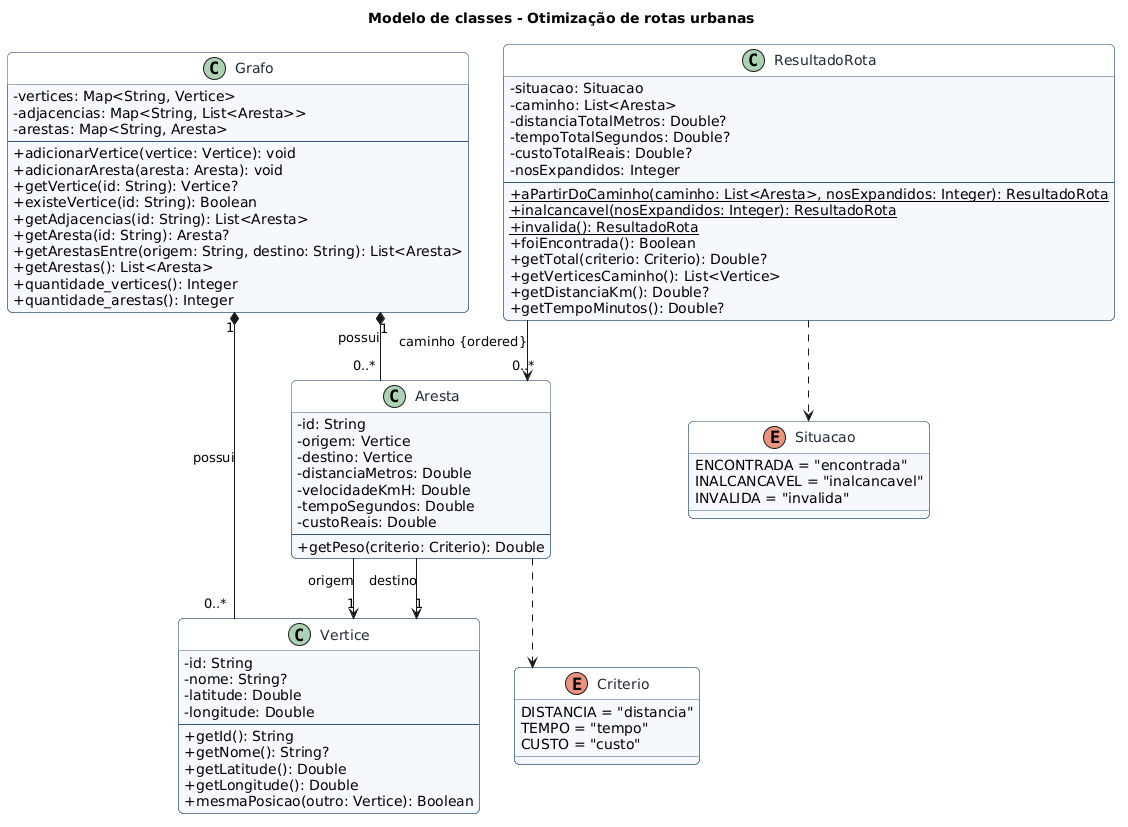
\includegraphics[width=0.95\textwidth, height=0.45\textheight, keepaspectratio]{diagramadeclassev3.png}
    \caption{Diagrama de classes UML.}
    \label{fig:diagrama-classes}
\end{figure}

A Figura~\ref{fig:diagrama-sequencia} representa a sequência de
interações envolvidas na solicitação de uma rota, desde a escolha dos
parâmetros pelo usuário até a apresentação do resultado.

\begin{figure}[H]
    \centering
    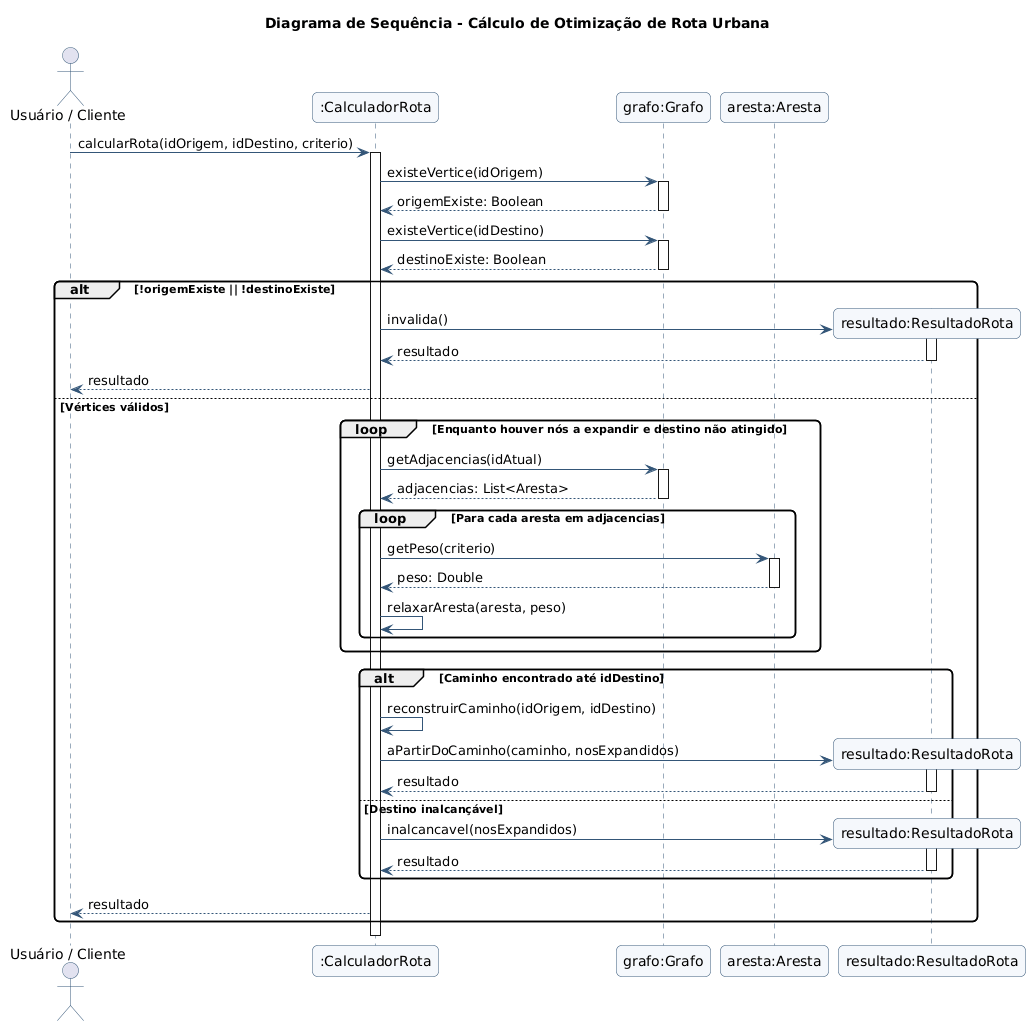
\includegraphics[width=0.9\textwidth, height=0.55\textheight, keepaspectratio]{diagramaSequencia3.png}
    \caption{Diagrama de sequência.}
    \label{fig:diagrama-sequencia}
\end{figure}

\section{Algoritmo e Implementação}
\label{sec:algoritmo}
Antes de calcular a rota, o usuário seleciona o algoritmo de busca e o
critério de otimização. O algoritmo escolhido determina como será
realizada a busca pelo caminho mínimo, enquanto o critério define o peso
utilizado em cada aresta: distância, tempo estimado ou custo financeiro.
Assim, a rota encontrada minimiza a soma dos pesos das arestas segundo o
critério selecionado.

A distância atribuída a cada aresta é estimada em metros pela fórmula de
Haversine entre as coordenadas geográficas de seus vértices extremos.
Como o snapshot não contém a geometria completa do traçado das ruas,
essa medida pode diferir do comprimento real do trecho. O tempo
estimado é calculado pela divisão da distância, em metros, pela
velocidade considerada para a via, convertida de quilômetros por hora
para metros por segundo:

\begin{equation}
    t = \frac{d}{v_{\text{km/h}} / 3{,}6}
    \label{eq:tempo}
\end{equation}

Quando a base de dados não informa a velocidade da via, o sistema utiliza
o valor padrão de $30\,\text{km/h}$.

O custo financeiro estimado considera um consumo médio de
$10\,\text{km/L}$ e o preço do combustível fixado em
$\text{R\$}\,5{,}80/\text{L}$. Com a distância expressa em metros, o
cálculo é:

\begin{equation}
    c = \left(\frac{d/1000}{10}\right) \times 5{,}80
    \label{eq:custo}
\end{equation}

Os dois algoritmos são implementados em Python no módulo
\texttt{rotas.py}. Dijkstra utiliza a fila de prioridade
\texttt{heapq}, além de um conjunto de vértices já processados. A
implementação ignora entradas desatualizadas da fila e encerra a busca
quando o destino é processado. Bellman-Ford percorre as listas de
adjacência dos vértices alcançáveis em passadas sucessivas, encerrando
antes de $|V|-1$ passadas se nenhuma estimativa for atualizada. Ao final,
verifica se ainda há uma aresta que poderia ser relaxada.

A seguir, os pseudocódigos resumem as operações principais. A validação
da solicitação e a reconstrução do caminho são funções compartilhadas
pelas duas implementações.

\subsection{Pseudocódigo de Dijkstra}

\begin{verbatim}
Dijkstra(G, origem, destino, peso):
    para cada vertice v em G:
        dist[v] <- infinito
        predecessor[v] <- indefinido
    dist[origem] <- 0
    fila <- [(0, origem)]
    processados <- conjunto vazio

    enquanto fila nao estiver vazia:
        (custo, u) <- remover menor elemento da fila
        se u em processados ou custo > dist[u]:
            continuar
        adicionar u a processados
        se u = destino:
            interromper

        para cada aresta (u, v) na lista de adjacencia de u:
            novo <- dist[u] + peso(u, v)
            se novo < dist[v]:
                dist[v] <- novo
                predecessor[v] <- aresta (u, v)
                inserir (novo, v) na fila

    reconstruir o caminho usando predecessor
\end{verbatim}

\subsection{Pseudocódigo de Bellman-Ford}

\begin{verbatim}
BellmanFord(G, origem, destino, peso):
    para cada vertice v em G:
        dist[v] <- infinito
        predecessor[v] <- indefinido
    dist[origem] <- 0

    repetir no maximo |V| - 1 vezes:
        alterou <- falso
        para cada vertice u alcancavel:
            para cada aresta (u, v) na lista de adjacencia de u:
                novo <- dist[u] + peso(u, v)
                se novo < dist[v]:
                    dist[v] <- novo
                    predecessor[v] <- aresta (u, v)
                    alterou <- verdadeiro
        se nao alterou:
            interromper

    se alguma aresta alcancavel ainda puder ser relaxada:
        indicar ciclo de peso negativo
    senao:
        reconstruir o caminho usando predecessor
\end{verbatim}

Na implementação atual, os pesos negativos são rejeitados pela classe
\texttt{Aresta}. Assim, a verificação de ciclo negativo existente em
Bellman-Ford não é acionada com os dados aceitos pelo modelo.

Com a fila de prioridade baseada em \texttt{heapq}, Dijkstra pode
inserir mais de uma estimativa para o mesmo vértice. Entradas antigas
são descartadas quando removidas da fila. Para essa implementação, o
tempo é $O(|V|+|E|\log |E|)$ no pior caso, e o espaço auxiliar é
$O(|V|+|E|)$, incluindo a fila. Bellman-Ford executa até
$|V|-1$ passadas pelas listas de adjacência e uma verificação adicional;
seu tempo no pior caso é $O(|V||E|)$ e seu espaço auxiliar é
$O(|V|)$.
\section{Interface}
\label{sec:interface}

A interface do sistema foi desenvolvida em Python com Streamlit, uma biblioteca para criação de aplicações web interativas. Para apresentar o mapa e desenhar os pontos de interesse e as rotas, foi utilizada a biblioteca Folium, integrada ao Streamlit pelo componente Streamlit-Folium.

A aplicação exibe um mapa centrado em Belo Horizonte e marca os pontos de interesse cadastrados. Na barra lateral, o usuário pode consultar locais pela API Nominatim do OpenStreetMap, salvar resultados no catálogo local, cadastrar um endereço manualmente por geocodificação ou remover um ponto cadastrado. A busca online é opcional; o mapa viário e o catálogo existentes são carregados de arquivos JSON locais.

Na tela principal, o usuário seleciona os pontos de origem e destino, escolhe o critério de otimização — distância, tempo ou custo — e seleciona o algoritmo: Dijkstra ou Bellman-Ford. Ao solicitar o cálculo, o aplicativo procura associar cada ponto de interesse ao vértice viário indicado no catálogo. Se esse identificador não existir no grafo, utiliza o vértice mais próximo das coordenadas do ponto. Como os identificadores atuais do catálogo não correspondem aos vértices do snapshot, as rotas envolvendo esses POIs são aproximações feitas sobre a malha local e não demonstram roteamento válido entre todas as regiões de Belo Horizonte. Em seguida, o aplicativo chama a função de busca do módulo \texttt{rotas.py}, usando o grafo montado por \texttt{mapa.py}.

Quando uma rota é encontrada, o sistema desenha no mapa o caminho formado pelos vértices do grafo e apresenta a distância total, o tempo estimado, o custo financeiro, o algoritmo utilizado e a quantidade de nós expandidos. Para solicitações inválidas ou destinos inalcançáveis, a interface exibe uma mensagem informativa. Os valores e o caminho apresentados são calculados pelo algoritmo com base nos dados do grafo; não são resultados simulados.

As principais bibliotecas utilizadas são:

\begin{itemize}
    \item \textbf{Streamlit}: criação dos controles interativos, organização da tela e exibição das métricas e mensagens;
    \item \textbf{Folium}: construção do mapa, marcadores dos pontos de interesse e desenho da rota;
    \item \textbf{Streamlit-Folium}: exibição e integração do mapa Folium na aplicação Streamlit;
    \item \textbf{Requests}: envio de consultas HTTP ao Nominatim para busca e geocodificação de locais;
    \item \textbf{JSON e bibliotecas padrão do Python}: leitura dos dados locais e coordenação entre interface, mapa, grafo e algoritmos.
\end{itemize}
 A Figura~\ref{fig:tela-principal} mostra a tela principal, com o mapa e os
controles disponíveis para selecionar os parâmetros da consulta. As
Figuras~\ref{fig:rota-bellman-ford-custo} e
\ref{fig:rota-dijkstra-custo} mostram exemplos de rotas calculadas com o
critério de custo, utilizando, respectivamente, os algoritmos de
Bellman-Ford e Dijkstra. Nessas telas, são exibidos o percurso no mapa e
as métricas retornadas pelo sistema.
\begin{figure}[htbp]
    \centering
    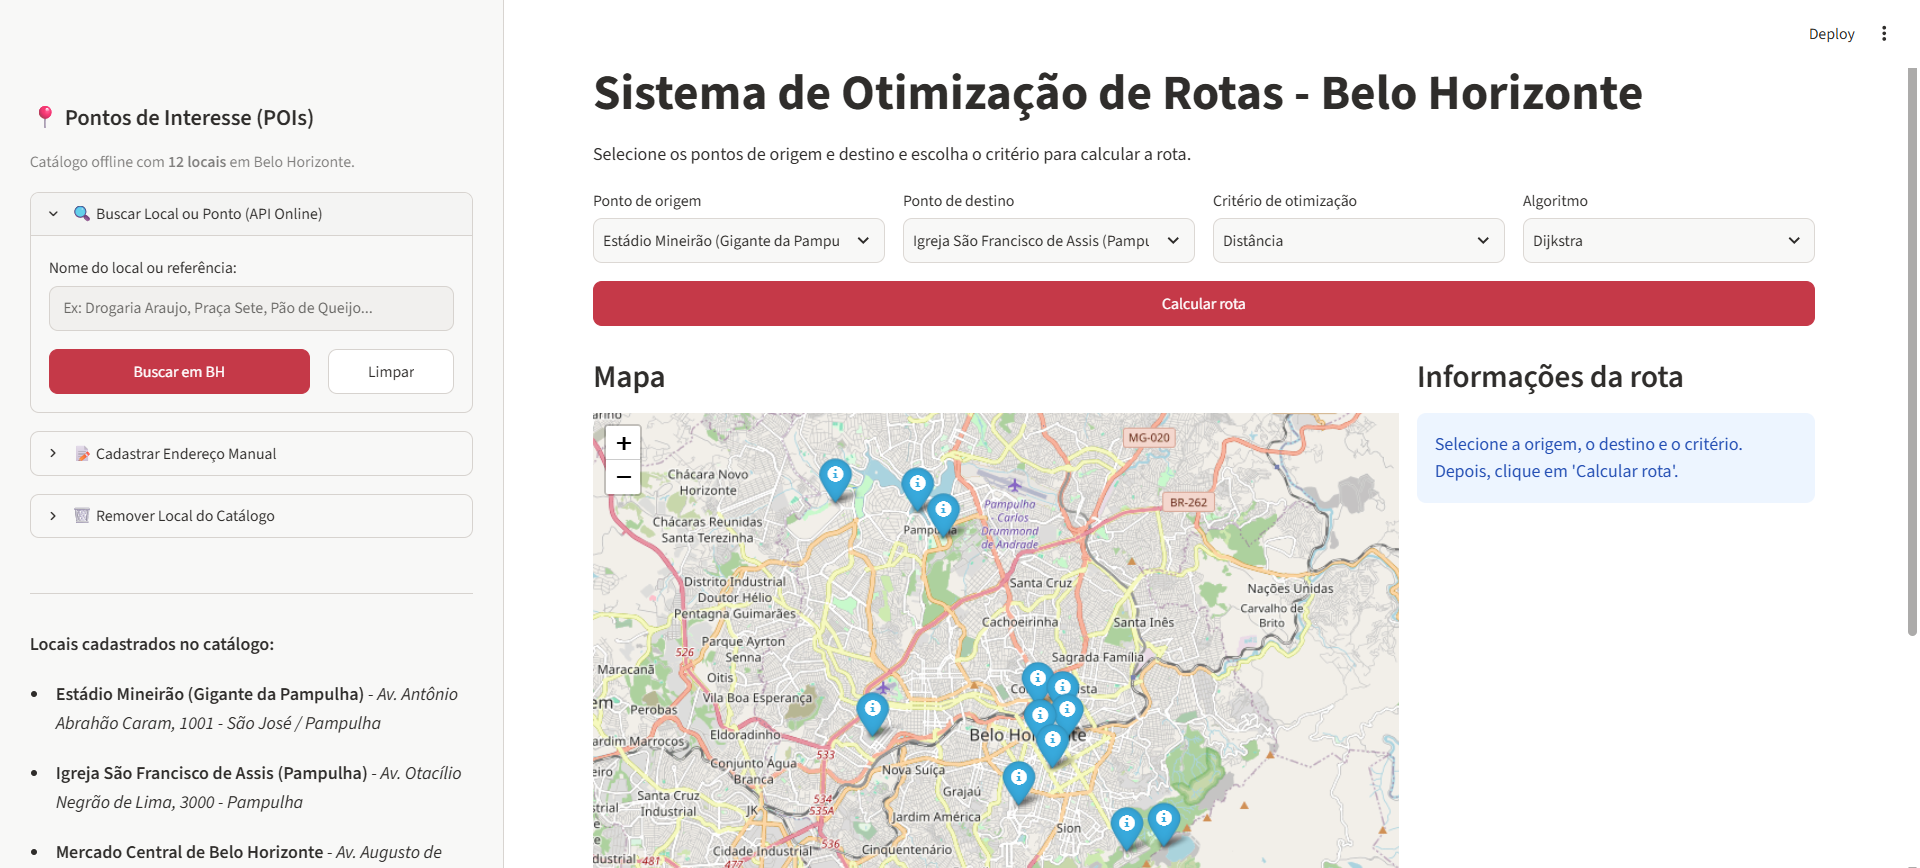
\includegraphics[width=0.95\textwidth, height=0.45\textheight, keepaspectratio]{tela.png}
    \caption{Tela principal da aplicação}
    \label{fig:tela-principal}
\end{figure}

\begin{figure}[htbp]
    \centering
    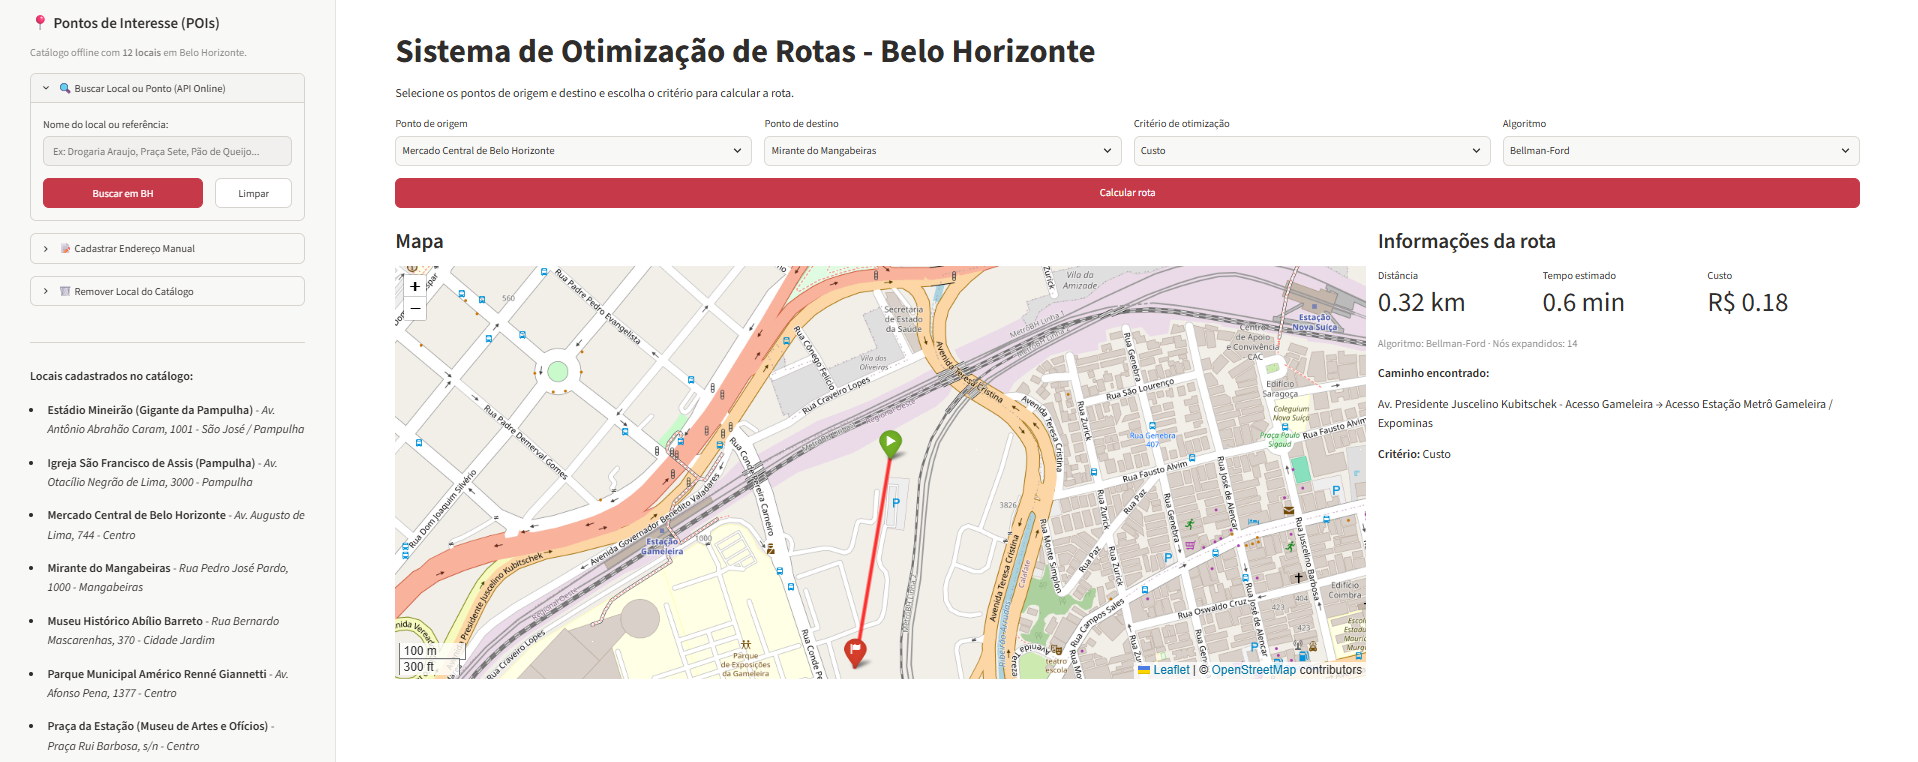
\includegraphics[width=0.95\textwidth, height=0.45\textheight, keepaspectratio]{tela2.png}
    \caption{Rota calculada com Bellman-Ford usando o critério de custo}
   \label{fig:rota-bellman-ford-custo}
\end{figure}
\begin{figure}[H]
    \centering
    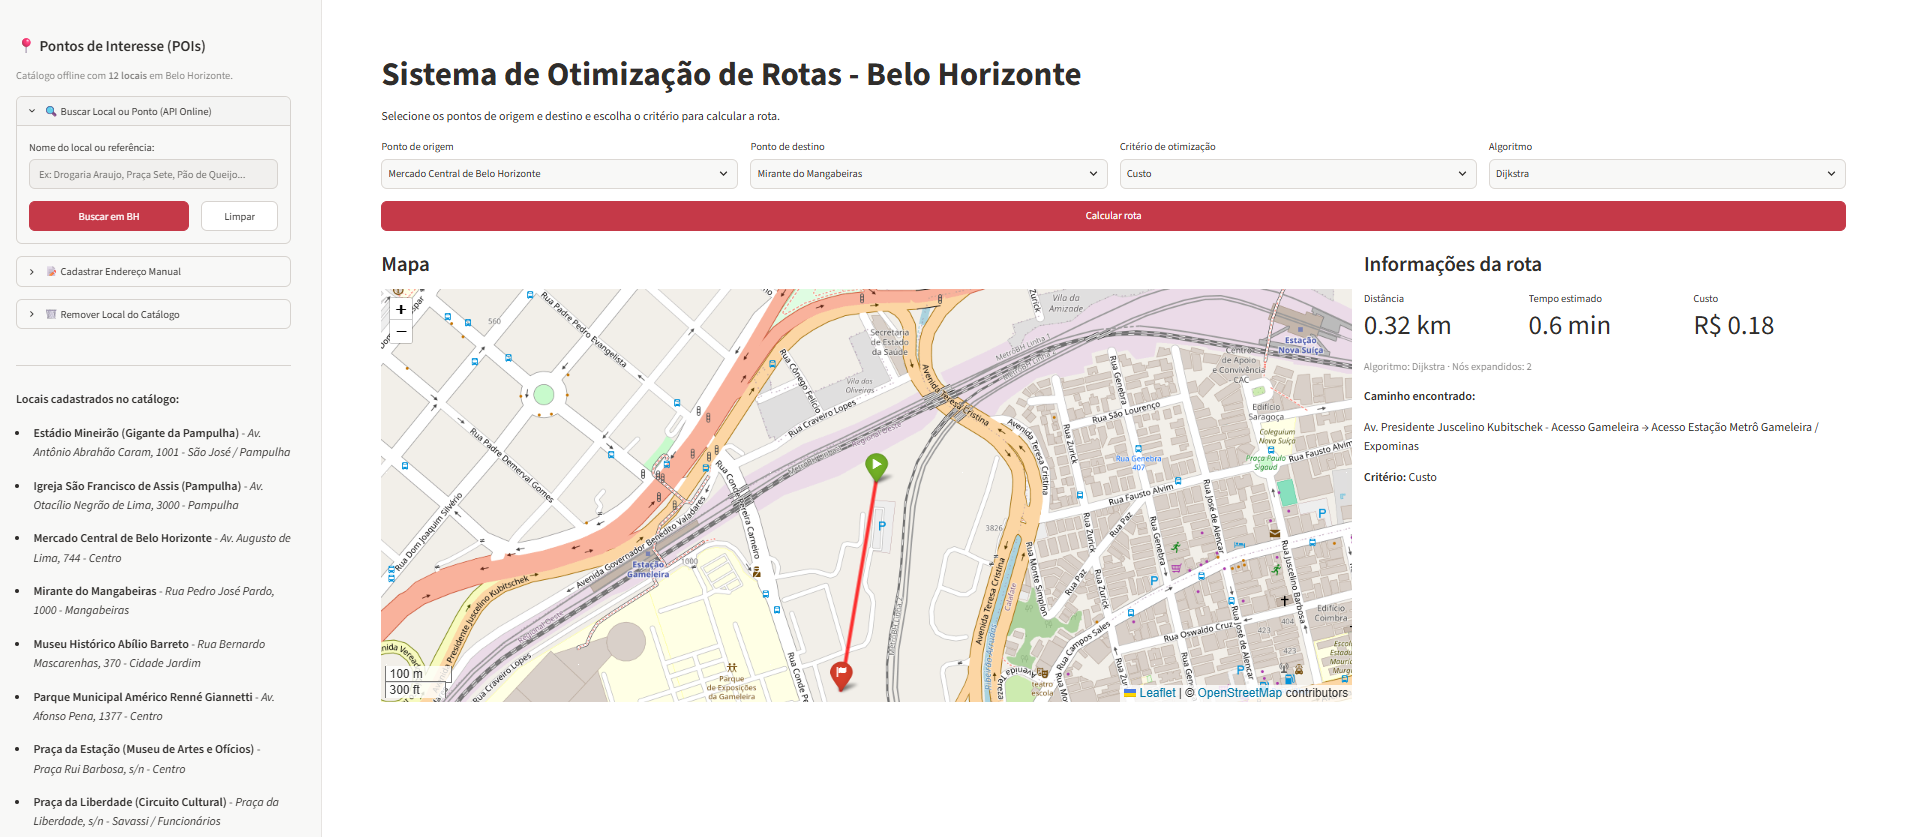
\includegraphics[width=0.95\textwidth, height=0.45\textheight, keepaspectratio]{tela3.png}
    \caption{Rota calculada com Dijkstra usando o critério de custo}
   \label{fig:rota-dijkstra-custo}
\end{figure}

\section{Avaliação Experimental e Comparação}
\label{sec:avaliacao}
\subsection{Protocolo experimental}
A comparação foi realizada sobre o snapshot local da malha viária,
composto por 34 vértices e 68 arestas direcionadas. Foram avaliados
os 1.122 pares ordenados distintos de origem e destino, considerando
os critérios de distância, tempo e custo. Para cada combinação de
par, critério e algoritmo, foi realizada uma execução de aquecimento
e 20 execuções cronometradas.

A medição utilizou \texttt{time.perf\_counter} e incluiu a busca e a
reconstrução do caminho, excluindo o carregamento dos dados e a
renderização da interface. Os resultados de Dijkstra e Bellman-Ford
foram comparados quanto à situação da busca e ao custo retornado. Os
1.122 pares ordenados possuem rota no grafo: mesmo respeitando a
orientação das vias de mão única, todo vértice alcança todos os
demais, ou seja, o grafo é fortemente conexo.

O benchmark foi executado em Windows 11 com Python 3.12.10, em um
processador AMD64 Family 25 Model 80 com 12 processadores lógicos.
A memória RAM não foi registrada e a máquina não estava isolada de
outras tarefas. Assim, as medições descrevem esse ambiente de execução.

\subsection{Resultados}
A Figura~\ref{fig:benchmark-tempo} apresenta o tempo mediano por busca.
Na distância, as medianas foram de 0,03010\,ms para Dijkstra e
0,13190\,ms para Bellman-Ford. No critério tempo, foram de 0,03060\,ms
e 0,13760\,ms, respectivamente. No custo, foram de 0,03070\,ms para
Dijkstra e 0,13880\,ms para Bellman-Ford.

Nos 1.122 pares, Dijkstra e Bellman-Ford retornaram o mesmo custo
mínimo nos três critérios. A mediana de vértices processados foi 18
para Dijkstra e 153,5 para Bellman-Ford. Essa
contagem não representa operações
equivalentes: Dijkstra conta vértices amadurecidos, enquanto
Bellman-Ford soma os vértices examinados nas passadas.

\begin{table}[ht]
\centering
\caption{Medianas de tempo e nós expandidos no snapshot local.}
\label{tab:benchmark}
\begin{tabular}{llrr}
\toprule
Critério & Algoritmo & Tempo mediano (ms) & Nós expandidos, mediana \\
\midrule
Distância & Dijkstra      & 0,03010 & 18    \\
Distância & Bellman-Ford  & 0,13190 & 153,5 \\
Tempo     & Dijkstra      & 0,03060 & 18    \\
Tempo     & Bellman-Ford  & 0,13760 & 153,5 \\
Custo     & Dijkstra      & 0,03070 & 18    \\
Custo     & Bellman-Ford  & 0,13880 & 153,5 \\
\bottomrule
\end{tabular}
\end{table}

\begin{figure}[H]
\centering
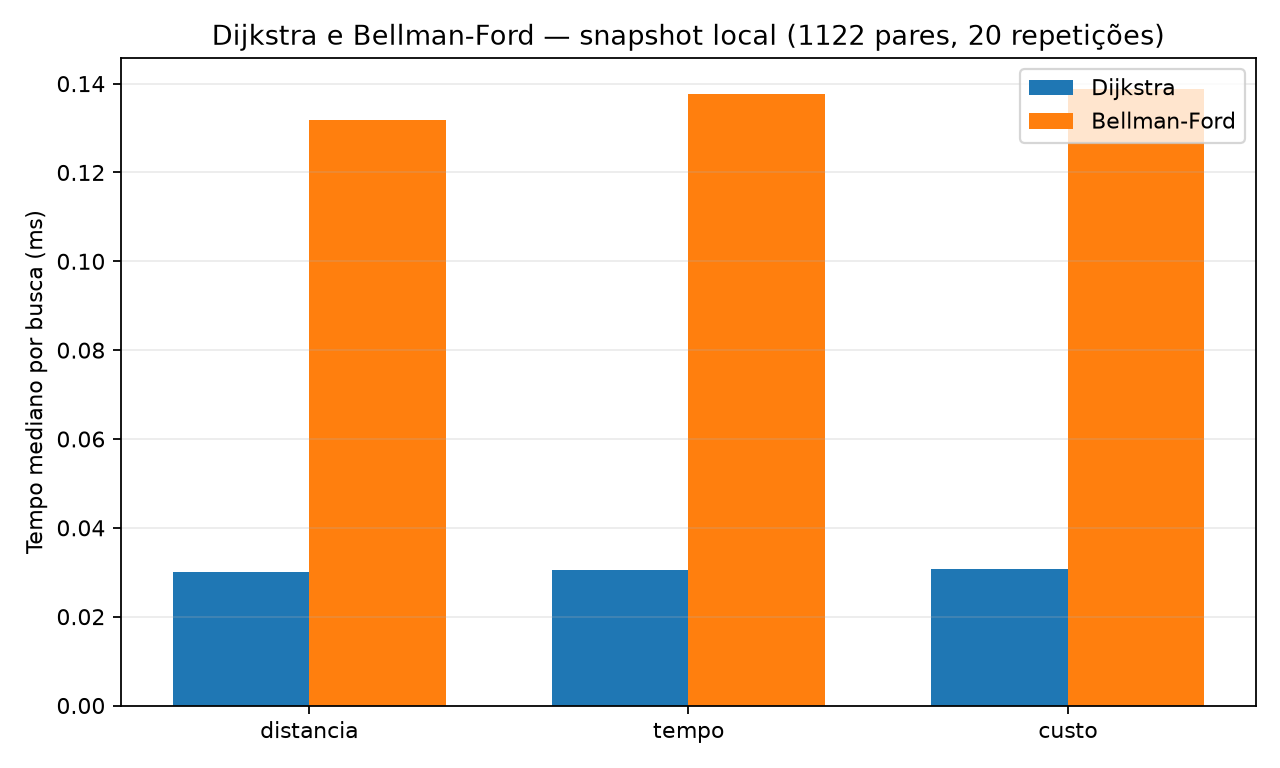
\includegraphics[width=0.95\linewidth]
{benchmark_tempo_mediano.png}
\caption{Tempo mediano de busca para cada critério no snapshot local.}
\label{fig:benchmark-tempo}
\end{figure}

\section{Discussão}
\label{sec:discussao}
Neste experimento, Dijkstra apresentou menores medianas de tempo nos
três critérios. Essa observação descreve apenas o snapshot avaliado:
as buscas foram muito curtas, e o ambiente de execução não estava
isolado de outras tarefas. Portanto, os valores não devem ser
generalizados para grafos maiores. Além disso, o número de nós
expandidos usa definições diferentes entre os algoritmos e não deve
ser interpretado como uma comparação direta da mesma quantidade de
operações.
\subsection{Limitações}
\label{subsec:limitacoes}

O sistema calcula rotas sobre um snapshot estático e local do bairro Coração Eucarístico. Embora o catálogo contenha pontos de interesse distribuídos por Belo Horizonte, os identificadores viários desses pontos não correspondem aos nós do snapshot; o vínculo pelo vértice mais próximo não permite interpretar as rotas resultantes como trajetos corretos entre regiões distantes da cidade. Os resultados também dependem da área coberta, da qualidade e da data dos dados e não refletem alterações posteriores nas ruas.

O modelo não considera condições de trânsito em tempo real, acidentes, obras, semáforos, horários de pico ou interdições temporárias. O tempo de percurso é estimado a partir da distância das vias e das velocidades registradas ou assumidas no conjunto de dados, portanto pode diferir do tempo observado durante uma viagem.

Os pontos de interesse são associados ao vértice viário mais próximo de suas coordenadas. Essa aproximação pode posicionar o início ou o fim da rota em um cruzamento próximo, em vez de representar exatamente o acesso ao local. A qualidade dessa associação depende da precisão das coordenadas e da densidade de vértices na região.

O custo financeiro também é uma estimativa. Seu cálculo usa parâmetros fixos de consumo e preço de combustível, sem considerar diferenças entre veículos, variações no preço da gasolina, pedágios, estacionamento ou outros gastos.

Como o consumo e o preço do combustível são constantes para todas as arestas, o custo calculado é proporcional à distância. Portanto, neste modelo, minimizar o custo financeiro produz o mesmo conjunto de rotas ótimas que minimizar a distância; o critério de custo não representa diferenças de consumo ou de preço entre trechos.

Por fim, a avaliação de desempenho realizada utiliza apenas o snapshot disponível, que contém 34 vértices e 68 arestas direcionadas. Portanto, os tempos medidos descrevem esse grafo pequeno e não permitem concluir, isoladamente, como os algoritmos se comportariam em redes viárias maiores. Os resultados também podem variar conforme o hardware e as condições de execução.

\section{Conclusão e Trabalhos Futuros}
\label{sec:conclusao}

Este trabalho desenvolveu um sistema de busca de rotas sobre um grafo
viário dirigido, com interface para seleção da origem, do destino, do
critério de otimização e do algoritmo de busca. O sistema contempla os
critérios de distância, tempo estimado e custo financeiro e implementa
Dijkstra e Bellman-Ford.

No benchmark realizado sobre o snapshot local, composto por 34 vértices
e 68 arestas direcionadas, os dois algoritmos encontraram os mesmos
custos para as consultas avaliadas. Nesse experimento, Dijkstra apresentou
menores tempos medianos nos três critérios. Esse resultado se limita ao
grafo e ao ambiente avaliados e não permite generalizações sobre redes
maiores.

Os pesos de tempo e custo são estimativas baseadas nas velocidades,
consumo e preço de combustível adotados. Além disso, a distância dos
trechos é calculada entre as coordenadas de seus vértices. Essas hipóteses
devem ser consideradas ao interpretar as rotas.

Como trabalhos futuros, propõe-se ampliar a avaliação para grafos maiores,
incluindo redes sintéticas e outros recortes viários; avaliar o comprimento
real da geometria das vias; estudar modelos de custo que variem por trecho;
e incorporar informações de trânsito e condições viárias mais detalhadas.

\subsection{Contribuições individuais}

As contribuições foram descritas a partir das alterações e dos commits
registrados no repositório.

\begin{itemize}
    \item Vinícius Simões: implementação da leitura dos dados do mapa,
    preparação dos pontos de interesse e testes relacionados à importação.
    \item Davi Soares: implementação e validação das estruturas do grafo
    e atualização do diagrama de classes.
    \item Áulus: implementação de Dijkstra e Bellman-Ford, testes de
    comparação e material de apoio para explicar os algoritmos.
    \item Pedro Matos: desenvolvimento da interface inicial com
    Streamlit e Folium.
    \item Maria Clara: documentação e diagramas, integração da interface
    com os algoritmos e preparação do script de benchmark.
    \item Henrique Neves: criação da suíte automatizada
    \texttt{codigo/test\_rotas.py}, com testes do modelo, da importação
    dos dados e dos algoritmos de rota, incluindo casos de borda e
    comparação com resultados conhecidos.

\end{itemize}

Todos os integrantes participaram da revisão final do artigo e da
preparação da apresentação.


\bibliographystyle{sbc}
\bibliography{sbc-template}
\section*{Declaração de uso de inteligência artificial}
Para a revisão textual deste artigo, foi utilizada a ferramenta
OpenAI Codex, baseada no modelo GPT-6 \cite{openaiCodex2026}.
\end{document}
